\documentclass[aspectratio=169]{beamer}

\usetheme{Madrid}
\usecolortheme{whale}
\usepackage[utf8]{inputenc}
\usepackage[T1]{fontenc}
\usepackage{amsmath,amssymb}
\usepackage{graphicx}
\usepackage{booktabs}
\usepackage{listings}
\usepackage{xcolor}

\graphicspath{{../../docs/mindmaps/}{../../docs/screenshots/}}

\definecolor{codegray}{gray}{0.95}
\definecolor{codeblue}{rgb}{0.1,0.1,0.6}
\definecolor{codegreen}{rgb}{0.0,0.5,0.0}
\lstset{
  basicstyle=\ttfamily\scriptsize,
  backgroundcolor=\color{codegray},
  language=Python, keywordstyle=\color{codeblue}\bfseries,
  commentstyle=\color{codegreen}\itshape, stringstyle=\color{purple},
  breaklines=true, columns=fullflexible, frame=single, framerule=0pt,
}

\title[SOEN 6011 --- D2 --- $B(x,y)$]{Deliverable 2 --- Function F6: Real Beta Function $B(x,y)$}
\subtitle{From-Scratch Implementation, Tkinter GUI, Repository, Updated Requirements}
\author[S. Bhowmik]{Shoban Bhowmik \quad (ID 40325778)}
\institute[Concordia]{SOEN 6011 --- Software Engineering Processes --- Section CC}
\date{2026-07-24 \quad (v0.2.0)}

\begin{document}

\begin{frame}\titlepage\end{frame}

% -------------------------------------------------------------------- outline
\begin{frame}{Outline}
  \begin{columns}[t]
    \column{0.5\textwidth}
    \begin{enumerate}
      \item What D2 adds
      \item From-scratch boundary (P5)
      \item Elementary functions
      \item Architecture \& exceptions
    \end{enumerate}
    \column{0.5\textwidth}
    \begin{enumerate}\setcounter{enumi}{4}
      \item Tkinter GUI \& errors
      \item Verification (P5)
      \item Repository (P6)
      \item Requirements v0.2 (P7) \& GAI (C-03)
    \end{enumerate}
  \end{columns}
\end{frame}

\begin{frame}{What Deliverable 2 adds}
Starting point (D1): Algorithm~B --- $B(x,y)=\exp\!\big(\ln\Gamma(x)+\ln\Gamma(y)-\ln\Gamma(x{+}y)\big)$,
a hand-written Lanczos $\ln\Gamma$, shipped as a CLI that borrowed only
$\ln,\exp,\sin,\pi$ from \texttt{math}.
\begin{itemize}
  \item \textbf{Problem 5 [60]} --- reimplement \emph{from scratch} (no math library) + a \textbf{Tkinter GUI}, with exception handling and helpful errors.
  \item \textbf{Problem 6 [20]} --- public Git repository, high-quality commits, README.
  \item \textbf{Problem 7 [20]} --- update the requirements from the D2 build.
\end{itemize}
\vfill
\footnotesize Domain $x>0,\,y>0$ (D-001). Individual work; CASTROFF GAI prompts logged (C-03).
\end{frame}

\begin{frame}{Problem 5 --- the ``from scratch'' boundary (D-008)}
Permitted: input, output, arithmetic, UI. Prohibited: every other library function.
The whole mathematical dependency was just four primitives:
\begin{center}\small
\begin{tabular}{@{}lll@{}}
\toprule
Borrowed (D1) & Role & Replacement (\texttt{elementary.py})\\
\midrule
\texttt{math.log} & logarithm & \texttt{ln}: mantissa reduction + atanh series\\
\texttt{math.exp} & exponential & \texttt{exp}: $k\ln2{+}r$ reduction + Taylor\\
\texttt{math.sin} & reflection & \texttt{sin}: argument reduction + Taylor\\
\texttt{math.pi} & constant & \texttt{PI}: correctly-rounded literal\\
\bottomrule
\end{tabular}
\end{center}
No \texttt{math.gamma}/\texttt{lgamma}/\texttt{beta} --- ever.
\textbf{IMPL-01} scans the shipped source and fails on any \texttt{math}/\texttt{numpy}/\texttt{scipy} import: it passes.
\end{frame}

\begin{frame}[fragile]{The elementary functions: reduce $\to$ series $\to$ rebuild}
\begin{lstlisting}
def ln(x):                      # x = m * 2**e,  m in [1/sqrt2, sqrt2)
    e = 0; m = x
    while m >= _SQRT2:  m *= 0.5; e += 1
    while m < _SQRT1_2: m *= 2.0; e -= 1
    s = (m-1)/(m+1); s2 = s*s     # |s| <= 0.1716 -> fast series
    term = s; total = s; denom = 1
    while True:                    # ln(m) = 2*(s + s^3/3 + s^5/5 + ...)
        term *= s2; denom += 2; d = term/denom; total += d
        if abs(d) < _EPS*abs(total)+_EPS: break
    return e*LN2 + 2*total
\end{lstlisting}
\footnotesize Verified vs.\ a trusted oracle: worst error $\exp\le6\times10^{-15}$, $\ln\le6\times10^{-16}$, $\sin\le9\times10^{-16}$.
Every loop is bounded (REL-03).
\end{frame}

\begin{frame}{Architecture + exception handling (D-011)}
\begin{columns}
\begin{column}{0.52\textwidth}
\textbf{Separation (testable core):}
\begin{itemize}\small
  \item \texttt{elementary.py} --- primitives
  \item \texttt{beta\_core.py} --- pure $\ln\Gamma,\beta$
  \item \texttt{validation.py} --- parsing + messages
  \item \texttt{gui.py} --- Tkinter only
\end{itemize}
\end{column}
\begin{column}{0.48\textwidth}
\textbf{Typed errors:} \texttt{BetaError}
\begin{itemize}\small
  \item \texttt{InputError} (empty/non-numeric/non-finite)
  \item \texttt{DomainError}, \texttt{RangeError}
  \item \texttt{NumericalRangeError}
\end{itemize}
\end{column}
\end{columns}
\vfill
\footnotesize Catch categories separately (ERR-02); one \texttt{except BetaError} guarantees no
traceback (REL-01). The core raises \texttt{NumericalRangeError} instead of returning
\texttt{inf}/\texttt{nan} (REL-02).
\end{frame}

\begin{frame}{Problem 5 --- the Tkinter GUI}
\begin{columns}
\begin{column}{0.56\textwidth}
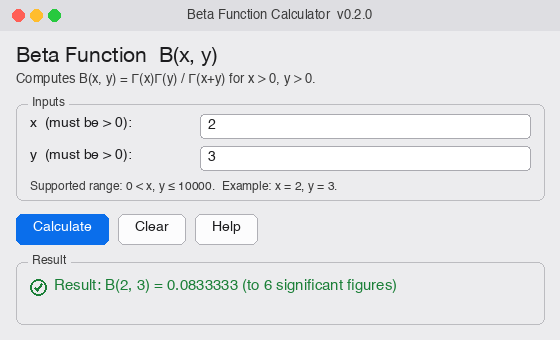
\includegraphics[width=\textwidth]{gui_valid.png}
\end{column}
\begin{column}{0.44\textwidth}\small
Wireframed first (D-010), traced to persona ``Maya''.
\begin{itemize}
  \item Labels state the domain: ``x (must be $>0$)''
  \item Keyboard-first: focus, Tab, \textsf{Enter}=calc, \textsf{Esc}=clear, \textsf{F1}=help (UI-01)
  \item Status is \emph{text} (a word + glyph), colour only redundant (ACC-03)
  \item Runs via \texttt{python3 src/gui.py} --- no IDE (POR-01)
\end{itemize}
\end{column}
\end{columns}
\end{frame}

\begin{frame}{Helpful errors, never a traceback (ERR-01, REL-01)}
\begin{center}
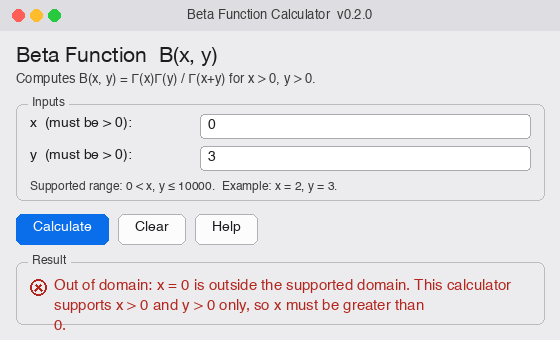
\includegraphics[width=0.62\textwidth]{gui_domain.png}
\end{center}
\footnotesize Each expected failure --- empty, non-numeric, out-of-domain, out-of-range,
numerical --- gets its own specific, corrective message. (Figures are layout renders of
\texttt{src/gui.py}, verified by GUI-01\dots06; the live window is shown in the demo.)
\end{frame}

\begin{frame}{Verification --- 27/27 (\texttt{tests/verify\_d2.py})}
\begin{itemize}
  \item \textbf{IMPL-01} shipped source imports no math library.
  \item \textbf{ACC-01} 18 reference values, worst relative error $\mathbf{1.17\times10^{-14}}$ --- \emph{identical to D1}: the from-scratch build cost nothing in accuracy.
  \item \textbf{VAL/ERR} five validation paths raise the right typed exception + helpful message.
  \item \textbf{REL-02} 36 large/small inputs all finite; \textbf{REL-03} bounded loops.
  \item \textbf{PERF-01} $7.8\times10^{-3}$\,ms/call; \textbf{POR-01} subprocess GUI launch.
  \item \textbf{GUI-01\dots06} handlers report the correct status for valid + each invalid case.
\end{itemize}
\centering\footnotesize Matrix: \texttt{docs/verification\_matrix\_d2.md}
\end{frame}

\begin{frame}{Problem 6 --- repository, commits, README}
\begin{itemize}
  \item Public Git host; URL recorded in the README (published from the author's account).
  \item \textbf{Incremental, high-quality history} (D-013): one cohesive change per commit,
        imperative subjects (``Add from-scratch elementary functions'', ``Add Tkinter GUI
        over the pure core'') --- not a single bulk upload.
  \item \texttt{.gitignore} excludes byte-code, \texttt{.DS\_Store}, \LaTeX{} artefacts, IDE settings, zips.
  \item \texttt{README.md}: purpose, exact run command, examples + screenshots, error guide,
        structure, version --- a new user can run it from the README alone.
\end{itemize}
\end{frame}

\begin{frame}{Problem 7 --- requirements v0.1 $\rightarrow$ v0.2 (D-012)}
All v0.1 IDs kept; changes discovered \emph{through implementation}:
\begin{center}\small
\begin{tabular}{@{}ll@{}}
\toprule
Change & Reason\\
\midrule
FR/USE/POR reworded & CLI $\rightarrow$ Tkinter GUI\\
VAL-02 & also reject \texttt{inf}/\texttt{nan}\\
ACC-03 promoted S$\rightarrow$M & accessibility is first-class\\
REL-02 explicit & raise \texttt{NumericalRangeError}\\
\textbf{+IMPL-01} & from-scratch mandate\\
\textbf{+UI-01} & keyboard operability\\
\textbf{+ERR-02} & typed input vs numerical errors\\
\bottomrule
\end{tabular}
\end{center}
\footnotesize 24 requirements; nothing deleted (superseded wording preserved). A-04/A-05 re-validated.
\end{frame}

\begin{frame}{GAI / CASTROFF evidence (C-03)}
\textbf{Tool:} Claude (Opus~4.8) via Claude Code. One CASTROFF prompt per problem
(TASK / RESTRICTIONS / OUTPUT FORMAT / AUDIENCE).
\begin{itemize}\small
  \item \textbf{P5:} generative + transformational --- boundary, primitives, GUI. \emph{Verified:} harness proved no library import + machine-precision primitives.
  \item \textbf{P6:} advisory --- \texttt{.gitignore}, commit plan, README. \emph{Adjusted:} publishing left to the author's account (outward-facing).
  \item \textbf{P7:} transformational + review --- evolved the baseline; each change tied to a matrix check + decision.
\end{itemize}
\footnotesize Every output critically evaluated (accepted/adjusted/rejected) and independently
verified. Logs: \texttt{docs/prompts/gai\_prompt\_log.md}.
\end{frame}

\begin{frame}{Limitations \& summary}
\textbf{Honest limitations:} domain $x,y>0$ only; magnitude cap $10^4$; very large
near-equal inputs underflow to $0.0$ (correct finite double); accuracy bounded by
Lanczos $g{=}7$; figures are renders (live window in demo).
\vfill
\textbf{Summary:} the Beta function is implemented \emph{from scratch} behind a Tkinter GUI
with typed exceptions and helpful messages; published with an incremental history and a
README; requirements updated to v0.2. \textbf{27/27} checks pass; accuracy unchanged at
$1.17\times10^{-14}$.
\vfill
\centering\small Demo: \texttt{python3 src/gui.py} --- $B(2,3)$, $B(0.5,0.5){=}\pi$, then $x{=}0$, $x{=}$``abc'', $x{=}10^6$.
\end{frame}

\begin{frame}{References}
\footnotesize
\begin{thebibliography}{9}
\bibitem{iso} ISO/IEC/IEEE 29148:2018 --- Requirements engineering.
\bibitem{lan} C.\ Lanczos, ``A Precision Approximation of the Gamma Function,'' 1964.
\bibitem{mul} J.-M.\ Muller, \emph{Elementary Functions: Algorithms and Implementation}, 3rd ed., 2016.
\bibitem{cw} W.\ Cody and W.\ Waite, \emph{Software Manual for the Elementary Functions}, 1980.
\bibitem{dlmf} NIST Digital Library of Mathematical Functions, \S5.12.
\bibitem{tk} Python Software Foundation, \emph{tkinter} documentation.
\end{thebibliography}
\vfill
\centering Thank you --- questions?
\end{frame}

\end{document}
